\documentclass[14pt, a4paper]{extreport}
\usepackage{susu}

% ====================================================================================================
\begin{document}

\author{Савонин~М.В.}
\group{211}
\task{6}
\maketitle

% ====================================================================================================
\chapter{Задание}

\begin{enumerate}

	\item
	Написать программу для построения гладкой кривой по четырем опорным точкам. При выборе опорных точек текущие координаты указателя мыши 	должны отображаться в графическом окне. Интерфейс программы должен содержать следующие элементы управления:
	\begin{itemize}
		\item выбор опорных точек;
		\item построение кубической кривой Безье;
		\item построение кривой по алгоритму Чайкина;
		\item сохранение результата в файл;
		\item выход из программы.
	\end{itemize}

\end{enumerate}

% ====================================================================================================
\chapter{Математическая модель}

\MakeUppercase{Кривая Безье}\\
Пусть x, y координаты центра, w, h длинна и ширина ромба, i номер угла и fi уголего наклона, то расчёт параметров ромба буду вычислять следующим способом.
Если мы нажали на угол ромба, то:\\
Если угол чётный то:
$$ r = (sqrt((mousex()-x)^2+(mousey-y)^2) - w)/2 .$$
$$ w = w + r .$$
Иначе:
$$ r = (sqrt((mousex()-x)^2+(mousey-y)^2) - h)/2 .$$
$$ h = h + r .$$
$$x = x+cos(fi+i*M_PI/2)*r.$$
$$y = y+sin(fi+i*M_PI/2)*r.$$
Иначе:
$$ x_{1} = mousex() - x.$$
$$ y_{1} = mousey() - y.$$
$$ fi = asin(y_{1} / (x_{1}*x_{1} + y_{1}*y_{1})^{1/2}) .$$
Если $x_{1}$ < 0:
$$ fi = M_PI - fi .$$
% ====================================================================================================
\chapter{Текст программы}

\noindent Файл main.cpp
\lstinputlisting{source/main.cpp}

% ====================================================================================================
\chapter{Результат работы}

\begin{figure}[h!]
	\centering
	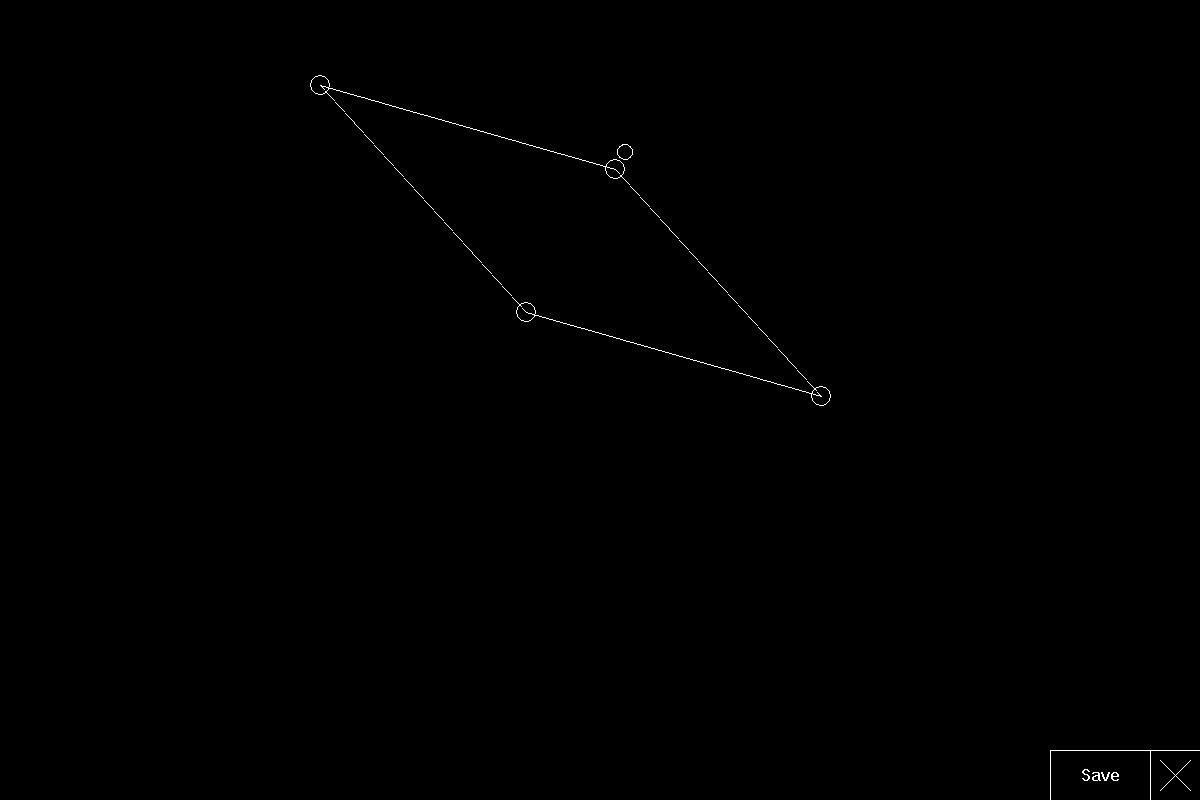
\includegraphics[width = 12cm]{image/output}
  \caption{Результат выполнения программы}
\end{figure}


% ====================================================================================================
\end{document}